\thispagestyle{empty}

% Title banner top
\AddToShipoutPicture*{%
 \AtPageUpperLeft{\raisebox{-\height}{\includegraphics{images/title-banner.png}}}}

% Report information
\begin{flushleft}
    \vspace{-10cm}
      $if(title)$
        {\relscale{2}{\textcolor{white}{$title$}}}\\ % HERE GOES THE TITLE OF THE DOCUMENT 
      $endif$
      \vspace{1cm} 
      
      $for(by-author)$
        {\relscale{1.5}{\textcolor{Yellow}{$by-author.name.literal$}}} % HERE GO THE AUTHORS
      $endfor$
    %\vspace{10cm}
\end{flushleft}
\begin{flushright}
    \vspace{-1cm}
        {\relscale{1.5}{\textcolor{Yellow}{Report}}}\\ % HERE GOES THE DOCUMENT TYPE
        \vspace{1cm}     
        {\relscale{1.5}{\textcolor{LightGray}{Report Date}}} % HERE GOES THE DATE OF PUBLICATION
\end{flushright}

% Cover picture
\vspace{0.5cm}
\begin{center}
  \makebox[\textwidth]{\includegraphics[width=\paperwidth]{images/cover-picture.jpg}}
\end{center}

% Title banner bottom 
\vspace{-15.5cm}
\begin{center}
  \makebox[\textwidth]{\includegraphics[width=\paperwidth]{images/title-banner-2.png}}
\end{center}

% Mobilizing Justice Logo
\vspace{1cm}
\begin{figure}[b]
\includegraphics[width=0.5\textwidth]{images/mj-logo.png}
\end{figure}

\onehalfspacing

\newpage

\section*{About Mobilizing Justice}

The Mobilizing Justice Partnership is funded by the Social Sciences and Humanities Research Council (SSHRC). Based at the University of Toronto Scarborough, the national intersectoral research partnership aims to understand and address transportation poverty in Canada and to improve the well-being of Canadians at risk of transport poverty. Learn more at \url{www.mobilizingjustice.ca}.

\section*{Our Partners}
\begin{center}
\ctable[
%label = width,
width = \textwidth,
pos = ht,
left,
doinside = \relscale{0.87}{}
]{| >{\setlength{\baselineskip}{0.1\baselineskip}}>{\raggedright}X | >{\setlength{\baselineskip}{0.1\baselineskip}}>{\raggedright}X | >{\setlength{\baselineskip}{0.1\baselineskip}}>{\raggedright}X |}{}
{ \FL
Amalgamated Transit Union Canada                                                & Infrastructure Canada              & Transit App                                \LL
Autorité régionale de transport métropolitain (ARTM)                            & McGill University                  & TransLink                      \LL
Canadian Institute of Planners                                                  & McMaster University                & United   Way Greater Toronto   \LL
Canada Mortgage and Housing Corporation (CMHC)                                  & Memorial University                & University of British Columbia \LL
Canadian Urban Institute                                                        & Metrolinx                          & University of Manitoba         \LL
Canadian Urban Transit Association                                              & Ontario Ministry of Transportation & University of Oregon           \LL
The Centre for Active Transportation (TCAT), a project of Clean Air Partnership & Pantonium                          & University of Texas Austin     \LL
CIRODD (École de technologie supérieure)                                        & Pembina Institute                  & University of Toronto          \LL
CIRRELT (Université de Montréal)                                                & Region of Waterloo                 & University of Waterloo         \LL
City of Calgary                                                                 & RideShark                          & Urban Strategies               \LL
City of Edmonton                                                                & Simon Fraser University            & Via Transportation Inc.        \LL
City of Toronto                                                                 & Spare Labs                         & Ville de Montréal              \LL
City of Vancouver                                                               & SPIN                               & York Region                    \LL
Esri Canada                                                                     & Statistics Canada                  &    \LL
Federation of Canadian Municipalities	& Toronto Transit Commission (TTC)	& \LL
}
\end{center}

\newpage

% TABLE OF CONTENTS
% Table of contents picture top
\AddToShipoutPicture*{%
 \AtPageUpperLeft{\raisebox{-\height}{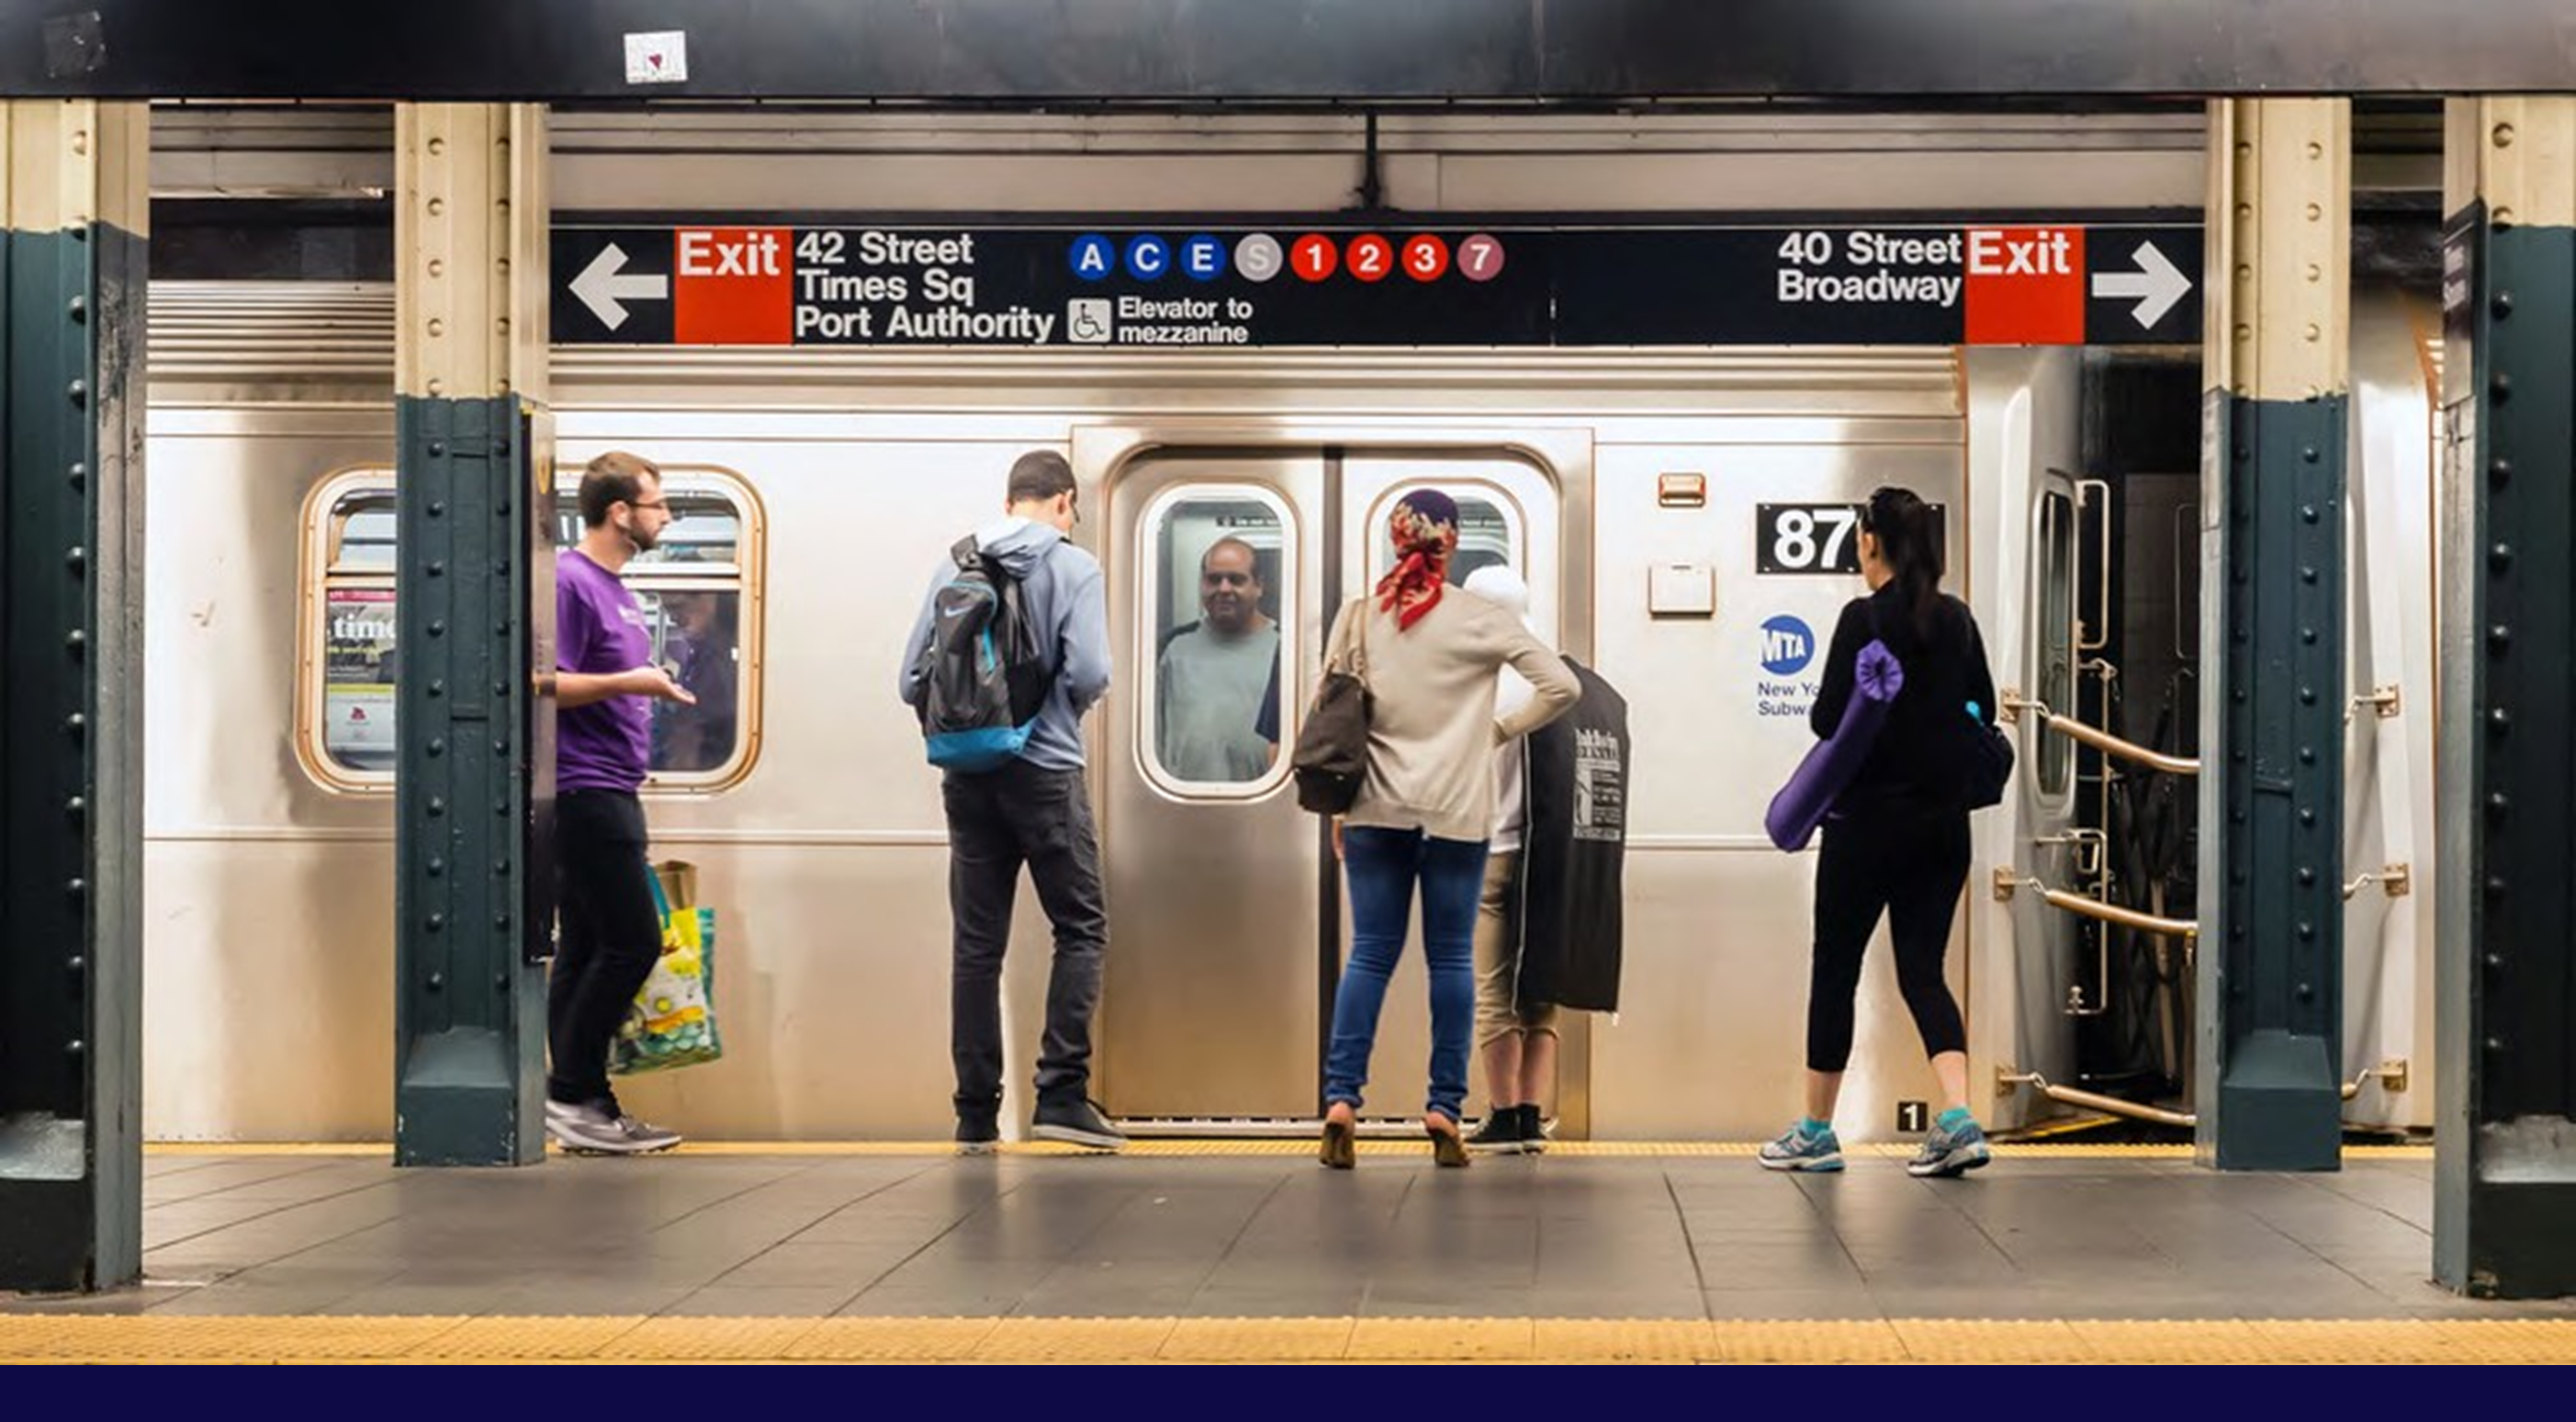
\includegraphics{images/table-of-contents-picture.png}}}}

%\begin{center}
%  \makebox[\textwidth]{\AddToShipoutPicture*{%
% \AtPageUpperLeft{\raisebox{-\height}{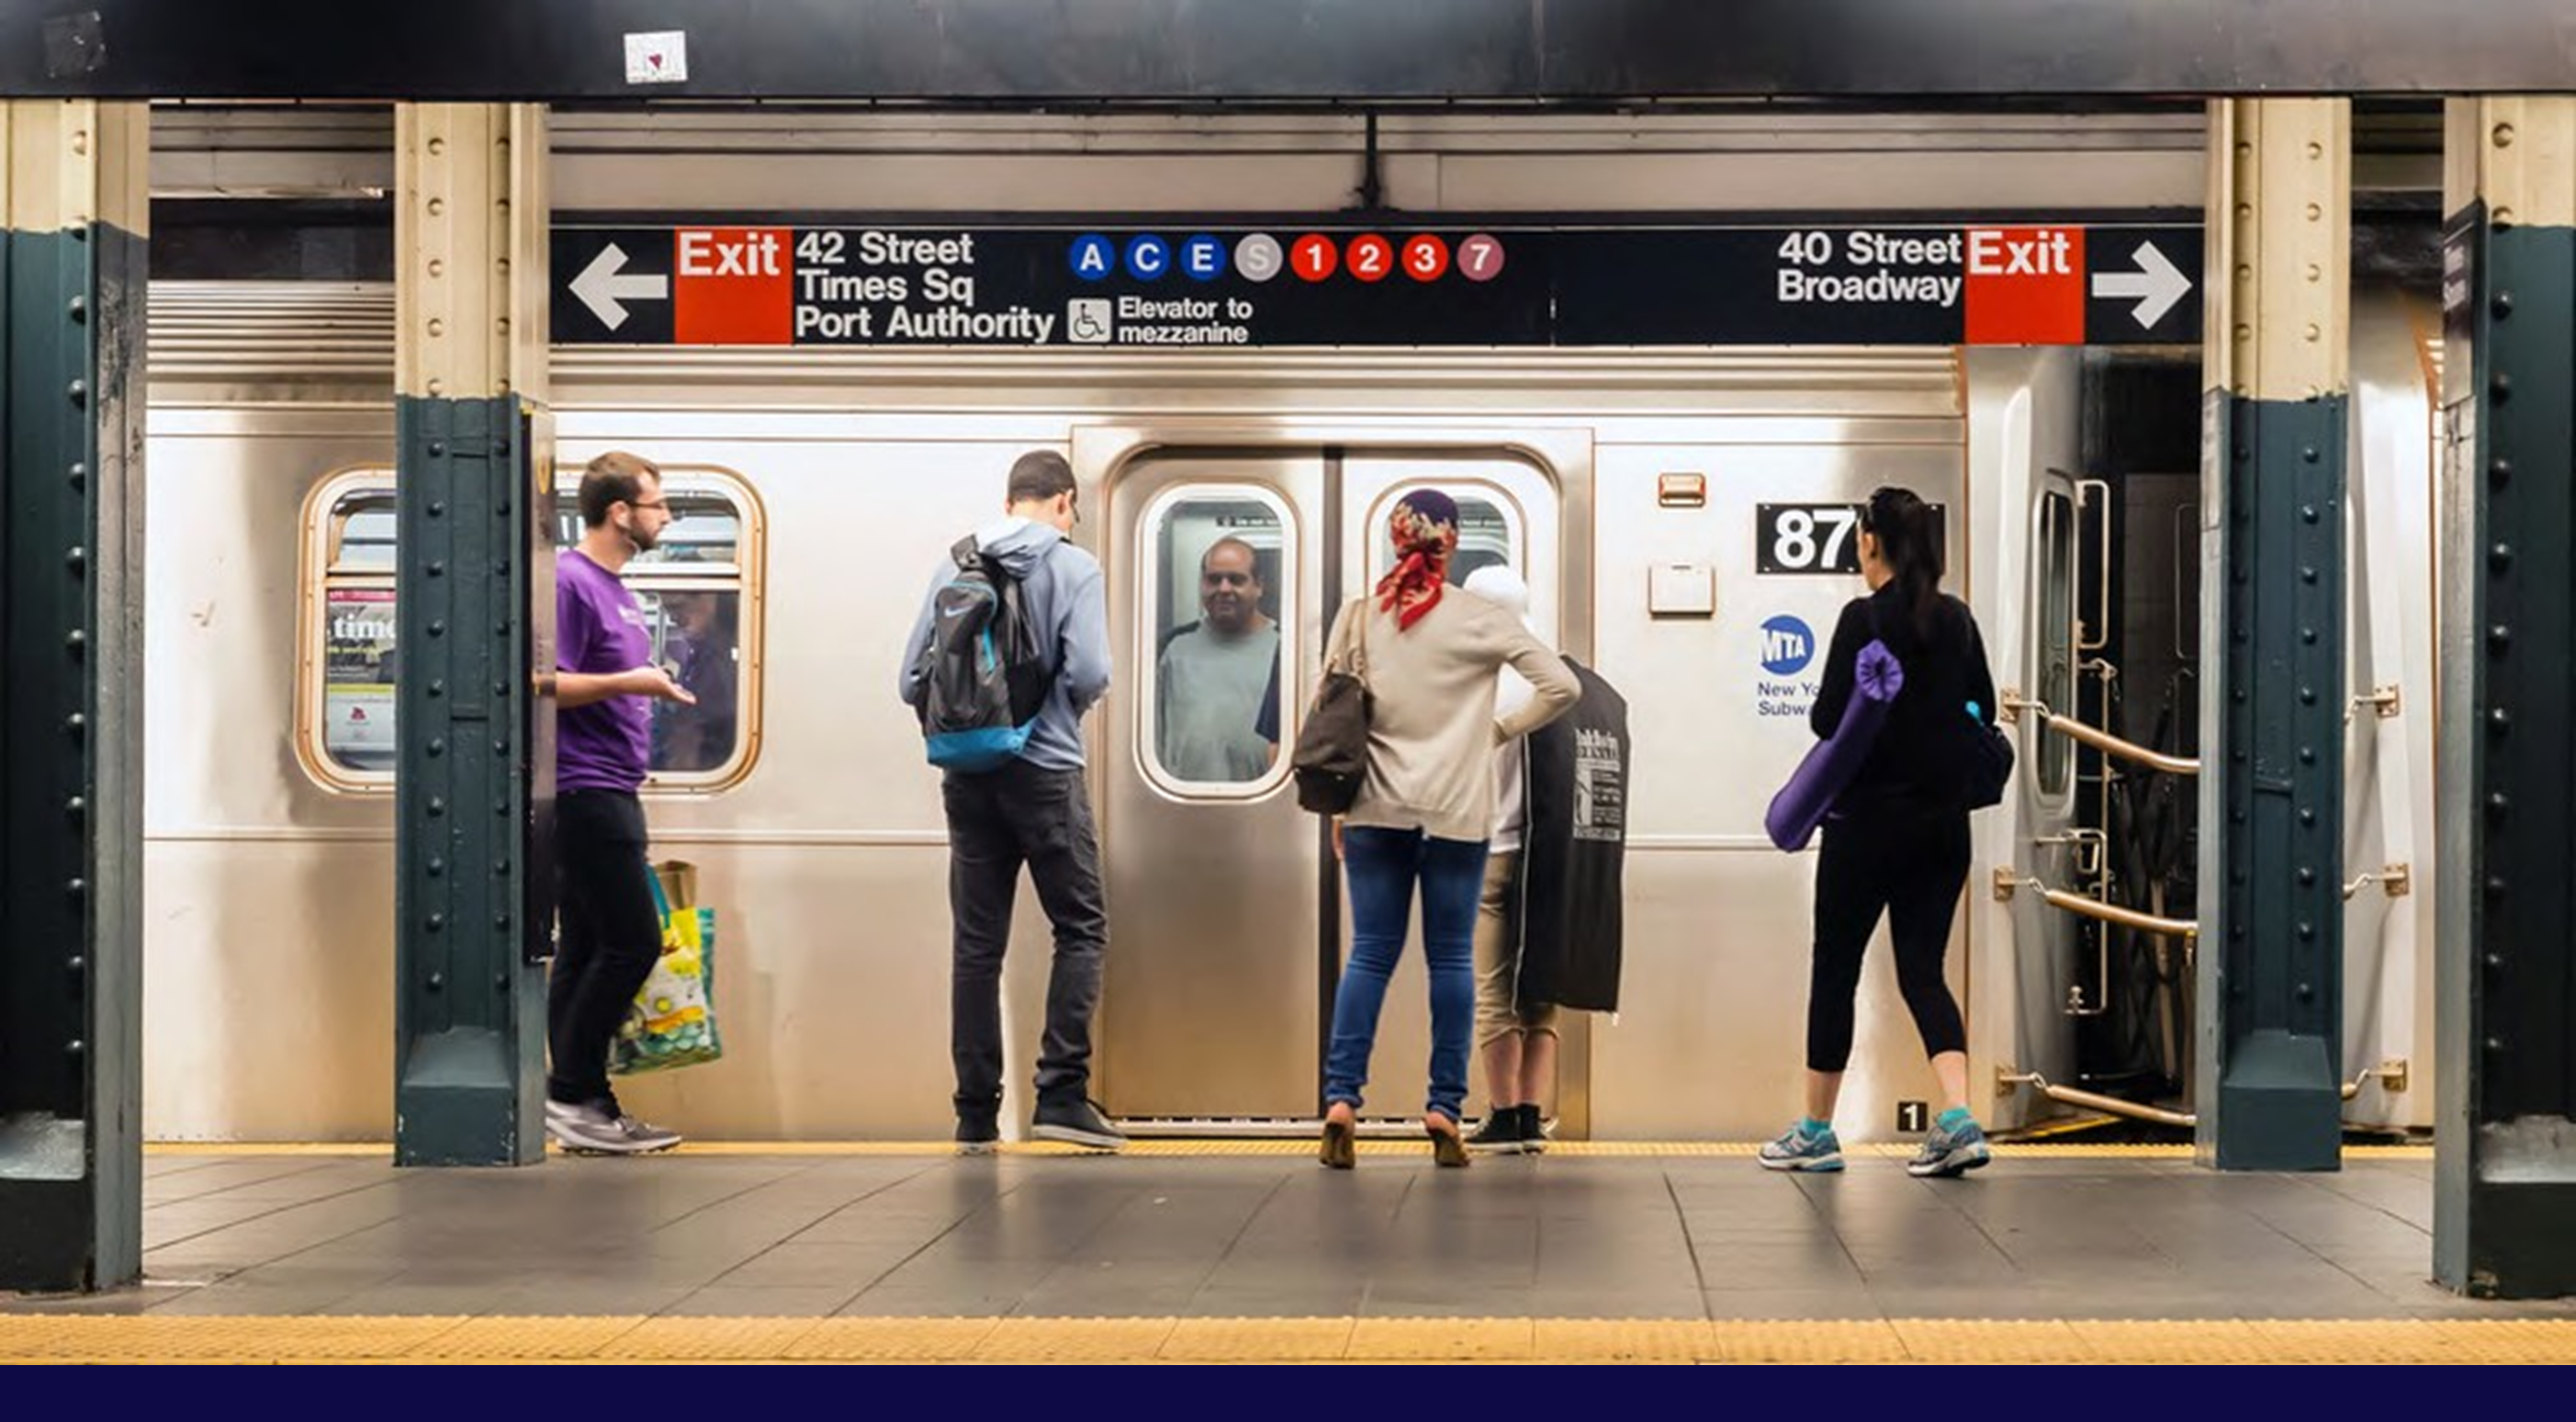
\includegraphics{images/table-of-contents-picture.png}}}}}
%\end{center}

% Change the geometry of the page for this one page, so that the table of contents is below the banner image instead of on top of it
\newgeometry{top=10cm}

% Title for the table of contents
\renewcommand\contentsname{\color{DarkBlue}\normalfont\bfseries\fontsize{24}{28.8}\selectfont Table of Contents}
%\restoregeometry
%\newgeometry{left=5cm}
\setcounter{tocdepth}{1}
\tableofcontents
\restoregeometry

\newpage